\documentclass{article}
\usepackage[T2A]{fontenc}
\usepackage{epigraph}
\usepackage[english, russian]{babel} % языковой пакет
\usepackage{amsmath,amsfonts,amssymb} %математика
\usepackage{mathtools}
\usepackage[oglav,spisok,boldsect,eqwhole,figwhole,hyperref,hyperprint,remarks,greekit]{../../style/fn2kursstyle}
\usepackage[utf8]{inputenc}
\usepackage[]{tkz-euclide}
\usepackage{algpseudocode}
\usepackage{pgfplots}
\usepackage{tikz-3dplot}
\usepackage[oglav,spisok,boldsect,eqwhole,figwhole,hyperref,hyperprint,remarks,greekit]{./style/fn2kursstyle}
\usepackage{multirow}
\usepackage{supertabular}
\usepackage{multicol}
\usepackage{tikz}
\usepackage{pgfplots}
\usepackage{float}
\usepackage{graphicx}
\pgfplotsset{compat=1.9}
\usepackage[svgnames]{pstricks}
\usepackage{pst-solides3d} 
\graphicspath{{../../style/}}
  



\newcommand{\cond}{\mathop{\mathrm{cond}}\nolimits}
\newcommand{\rank}{\mathop{\mathrm{rank}}\nolimits}
% Переопределение команды \vec, чтобы векторы печатались полужирным курсивом
\renewcommand{\vec}[1]{\text{\mathversion{bold}${#1}$}}%{\bi{#1}}
\newcommand\thh[1]{\text{\mathversion{bold}${#1}$}}
%Переопределение команды нумерации перечней: точки заменяются на скобки
\renewcommand{\labelenumi}{\theenumi)}
\newtheorem{theorem}{Теорема}
\newtheorem{define}{Определение}
\tdplotsetmaincoords{60}{115}
\pgfplotsset{compat=newest}

\title{Прямые методы решения систем
линейных алгебраических уравнений}
\author{Н.\,О.~Акиньшин}
\group{ФН2-51Б}
\date{2024}
\supervisor{А.\,С.~Джагарян}



\begin{document}
    \maketitle
    \newpage
    \tableofcontents
    \newpage

    \section{Исходные данные}
    \begin{enumerate}
        \item Тестовый пример 1
        \begin{equation}
            \begin{dcases}
                x_1 + x_2 + x_3 + x_4 = 4, \\
                    x_2 + x_3 + x_4 = 3, \\ 
                        x_3 + x_4 = 2, \\
                            x_4 = 1.
            \end{dcases}
        \end{equation}
        Точное решение: $x = (1, 1, 1, 1)^T$. \newline
        $\cond_1 A = 8, \  \cond_\infty A = 8$
        \item Тестовый пример 2
            \begin{equation}
                \begin{dcases}
                    x_4 = 1, \\
                    x_3 + x_4 = 2, \\
                    x_2 + x_3 + x_4 = 3, \\ 
                    x_1 + x_2 + x_3 + x_4 = 4. \\
                \end{dcases}
            \end{equation}
            Точное решение: $x = (1, 1, 1, 1)^T$. \newline
            $\cond_1 A = 8, \  \cond_\infty A = 8$
        \item Тестовый пример 3
            \begin{equation}
                \begin{dcases}
                    x_1 + x_2 + x_3 + x_4 = 4, \\ 
                    2x_1 + 3x_2 + 3x_3 + 3x_4 = 11, \\ 
                    2 x_1 + 4x_2 + 4x_3 + 4x_4 = 15, \\ 
                    4 x_1 + 5 x_2 + 6 x_3 + 7 x_4 = 22
                \end{dcases}
            \end{equation}
        Матрица не совместна, $\cond A = \infty$.
        \item Тестовый пример 4
        \begin{equation}
            \begin{dcases}
                10x_1 + 6x_2 + 2x_3 = 25, \\
                5x_1  + x_2 - 2x_3 + 4x_4 = 14, \\ 
                3x_1 + 5x_2 + x_3 - x_4 = 10, \\
                6x_2 -2x_3 +2x_4 = 8
            \end{dcases}
        \end{equation}
        Точное решение: $x = (2, 1, -0.5, 0.5)^T$. \newline
            $\cond_1 A \approx 240.55, \  \cond_\infty A \approx 269.19$
        \item Тестовый пример 5
        \begin{equation}
            \begin{dcases}
                28.589x_1 -0.008x_2+ 2.406x_3+ 19.24x_4 = 30.459, \\ 
                14.436x_1 -0.001x_2 + 1.203x_3 + 9.624x_4 = 18.248, \\
                120.204x_1 -0.032x_2 + 10.024x_3 +  80.144x_4 = 128.156, \\
                -57.714x_1 + 0.016x_2 -4.812x_3 -38.478x_4 = -60.908.
            \end{dcases}
        \end{equation}
        Точное решение: $x = (1, 1000, -20, 3)^T$. \newline
            $\cond_1 A \approx 122414849.9, \  \cond_\infty A \approx 109686235.3.$
        \item Система варианта 1
        \begin{equation}
            \begin{dcases}
                16.3820x_1 -2.0490x_2 -41.8290x_3 + 16.3920x_4 = 33.6130\\
                307.6480x_1 -38.4660x_2 -840.3660x_3 + 312.5280x_4 = 710.3420 \\
                0.4560x_1 -0.0570x_2 -1.1770x_3 + 0.4560x_4 = 0.9490 \\ 
                23.2720x_1 -2.9090x_2 -66.3090x_3 + 23.8720 = 57.6730
            \end{dcases}
        \end{equation}
        \item Система варианта 2
        \begin{equation}
            \begin{dcases}
                31.2000x_1 -1.3200x_2 -7.6800 x_3 + 4.0900 x_4 = -83.3200 \\
                7.2300 x_1 -126.0000 x_2 + 7.1400 x_3 + 3.0400 x_4 = 38.9000 \\ 
                9.4900 x_1 + 6.4000 x_2 + 6.0000 x_3 + 8.4500 x_4 = -56.7000 \\ 
                2.6800 x_1 -3.2900 x_2 + 0.2800 x_3 + 13.4000 x_4 = -504.0900
            \end{dcases}
        \end{equation}  
    \end{enumerate}

\section{Краткое описание используемых алгоритмов}
\subsection{Метод Гаусса}
Метод Гаусса --- это алгоритм решения систем линейных уравнений. 
Основная идея заключается в преобразовании системы уравнений к треугольному виду с 
помощью элементарных преобразований строк матрицы, а затем нахождении решения методом обратного 
хода.
\subsection{QR-разложение}
QR-разложение --- это метод разложения матрицы на произведение двух матриц: ортогональной матрицы 
Q и верхнетреугольной матрицы R.
\section{Контрольные вопросы}
\begin{enumerate}
    \item Каковы условия применимости метода Гаусса без выбора
    и с выбором ведущего элемента?
    \newline
    {\bfseries Ответ}.
    Метод Гаусса может быть реализован, когда все числа $a_{11},\, a_{22}^{(1)},\, \ldots,\, a_{nn}^{(n-1)}$ отличны от нуля. Введем обозначения $A_1, \, A_2,\, A_n$ -- главные миноры матрицы системы.
	\[
	A_1 = a_{11}, \, A_2 = \begin{bmatrix}
		a_{11} & a_{12}\\
		a_{21} & a_{22}
	\end{bmatrix}, \, A_n = \begin{bmatrix}
	a_{11} & a_{12} & \ldots & a_{1n}\\
	a_{21} & a_{22} & \ldots & a_{2n}\\
	\ldots & \ldots & \ldots & \ldots\\
	a_{n1} & a_{n2} & \ldots & a_{nn} 
	\end{bmatrix}
	\]
	
	
	\textbf{Теорема.} Для того, чтобы все ведущие элементы метода Гаусса были отличны от нуля необходимо и достаточно, чтобы все главные миноры матрицы A были ненулевыми.
	
	
	\textbf{Доказательство}.
	
	
	Достаточность. Пусть все главные миноры матрицы A отличны от нуля. Доказательство будем проводить по индукции.
	
	
	\noindent1) База индукции $a_{11} = A_1 \neq 0 $
	
	
	\noindent2) Предположим, что $a_{11},\, a_{22}^{(1)},\, \ldots, \, a_{k-1 k-1} ^ {(k-2)} \neq 0$. Покажем, что $a_{k k} ^ {(k-1)} \neq 0$. Приведем минор $A_k$ к верхне треугольному виду при помощи прямого ходу метода Гаусса. В ходе таких преобразований определитель может изменить только свой знак.
	
	\begin{equation}
		\label{minor}
		A_k = a_{11} \cdot a_{22}^{(1)} \ldots a_{k-1 k-1} ^ {(k-2)} \cdot \begin{bmatrix}
			1 & a_{12}^{(1)} & \ldots & a_{1k}^{(1)}\\
			0 & 1 & \ldots & a_{2k}^{(2)}\\
			\ldots & \ldots & \ldots & \ldots\\
			a_{n1} & a_{n2} & \ldots & a_{kk}^{(k-1)} 
		\end{bmatrix} = a_{11} \cdot a_{22}^{(1)} \ldots a_{k-1 k-1} ^ {(k-2)} \cdot a_{kk}^{(k-1)}.
	\end{equation}

	Поскольку $A_k \neq 0$ и по предположению  $a_{11},\, a_{22}^{(1)},\, \ldots, \, a_{k-1 k-1} ^ {(k-2)} \neq 0$, то из формулы \ref{minor} следует, что$a_{kk}^{(k-1)} \neq 0$. ч.т.д
	
	
	Необходимость. Очевидно следует из формулы \ref{minor}
    \item Докажите, что если $\det A \neq 0$, то при выборе
    главного элемента в столбце среди элементов, лежащих не выше главной диагонали,
    всегда найдется хотя бы один элемент, отличный от нуля.
    \newline
    {\bfseries Доказательство}. 
    Докажем методом математической индукции.
    \newline 
    {\bfseries База индукции}. Рассмотрим матрицу $2 \times 2$. 
    \begin{equation*}
        A_2 = 
      \begin{pmatrix}
        a_{11} & a_{12} \\ 
        a_{21} & a_{22}
      \end{pmatrix}
    \end{equation*}
    Тогда $\det A \neq 0$, то есть матрица не имеет нулевых строк и столбцов. Это верно, в случае
    если $a_{22} \neq 0$ и ($a_{11} \neq 0$ или $a_{21} \neq 0$), то есть существует хотя бы 
    1 элемент в каждом столбце, который отличен от нуля и находится не выше главной диагонали.
    
    
    {\bfseries Переход индукции}. Пусть для матрицы $A_n$ верно, что при 
    $\det A_n \neq 0$ следует отличие от нуля хотя бы одного элемента в каждом столбце 
    не выше главной диагонали. Тогда по методу Гаусса приведем матрицу к верхнетреугольному виду, разместив 
    эти элементы на главной диагонале.
    \begin{equation*}
      \widetilde{A_n} = 
      \begin{pmatrix}
        a_{11} & a_{12} & \dots & a_{1n} \\
        0 & a_{22} & \dots & a_{2n} \\
        \vdots \\ 
        0 & 0 & \dots & a_{nn}
      \end{pmatrix}
    \end{equation*}
    Расширим матрицу $\widetilde{A_n}$ до $A_{n+1}: (n+1) \times (n+1)$, причем 
    $\det A_{n+1} \neq 0$
    Тогда матрица примет следующий вид:
    \begin{equation*}
      A_{n+1} = 
      \begin{pmatrix}
        a_{11} & a_{12} & \dots & a_{1n} & a_{1 (n+1)}\\
        0 & a_{22} & \dots & a_{2n} & a_{2 (n+1)} \\
        \hdotsfor[3]{5} \\ 
        0 & 0 & \dots & a_{nn} & a_{n (n+1)} \\ 
        a_{(n+1) 1} & a_{(n+1) 2} & \dots & a_{(n+1) n}& a_{(n+1) (n+1)}
      \end{pmatrix}
    \end{equation*}
    По методу Гаусса обнулим первые $n$ столбцов $n+1$ строки.
    \begin{equation*}
        \widetilde{A_{n+1}} = 
        \begin{pmatrix}
          a_{11} & a_{12} & \dots & a_{1n} & a_{1 (n+1)}\\
          0 & a_{22} & \dots & a_{2n} & a_{2 (n+1)} \\
          \hdotsfor[3]{5} \\ 
          0 & 0 & \dots & a_{nn} & a_{n (n+1)} \\ 
          0 & 0 & \dots & 0& \tilde{a}_{(n+1) (n+1)}
        \end{pmatrix}
      \end{equation*}
    Заметим, что $\det \widetilde{A_{n+1}} \neq 0 \Leftrightarrow  a_{(n+1) (n+1)} \neq 0$.
    Тогда по методу математической индукции утверждение доказано для любого натурального $n \geqslant 2$.
    \item В методе Гаусса с полным выбором ведущего элемента
    приходится не только переставлять уравнения, но и менять нумерацию неизвестных. 
    Предложите алгоритм, позволяющий восстановить первоначальный порядок неизвестных.
    \newline
    {\bfseries Ответ}.
    Будем хранить перестановку переменных $x_i \rightarrow x_j$ в виде $(i, j)$.
    Тогда создадим переменную $permutations$, которая будет хранить все перестановки.

    В общем виде:
    \begin{equation*}
        permutations = ((n_1, n_2), (n_3, n_4), \ldots, (n_{k-1}, n_k)),
    \end{equation*}
    где $n_i$ - порядковый номер переменной.
    При добавлении новой нумерации двух переменных следует записать их в конец $permutations$.
    Для восстановления порядка, необходимо проделать замены в обратном порядке, записанном в $permutations$:
    \begin{equation*}
        recover = ((n_k, n_{k-1}), (n_{k-2}, n_{k-3}), \ldots, (n_2, n_1)).
    \end{equation*}
    Выполняя замены, записанные в $recover$, можно получить изначальный порядок переменных.
    \item Оцените количество арифметических операций, требуемых для QR-разложения произвольной матрицы $A$ размера $n\times n $.
    \newline
    {\bfseries Ответ}.
    Оцените количество арифметических операций, требуемых
	для QR-разложения произвольной матрицы A размера n×n.
	
	Для того, чтобы подсчитать количество операций рассмотрим псевдокод QR-разложения.
	
	
	\noindent QRDecomposition(size, Matrix, TMatrix)
	\begin{algorithmic}[1]
		\For{i=0 ; i < size-1; i++}
			\For{j=i+1; j < size-1; j++}
				\If{Matrix[j][i]==0}
					\State continue
				\EndIf
				\State c = Matrix[i][i] / sqrt(Matrix[i][i] * Matrix[i][i] + Matrix[j][i] * Matrix[j][i])
				\State s = Matrix[j][i] / sqrt(Matrix[i][i] * Matrix[i][i] + Matrix[j][i] * Matrix[j][i])
				\For{k=0; k < size+1; k++}
					\State tmp1 = Matrix[i][k] * c + Matrix[j][k] * s
					\State tmp2 = Matrix[j][k] * c - Matrix[i][k] * s
					
					\State Matrix[i][k] = tmp1
					\State Matrix[j][k] = tmp2
				\EndFor
				
				\For{k=0; k < size; k++}
				\State tmp3 = c * TMatrix[i][k] + s * TMatrix[j][k]
				\State tmp4 = -s * TMatrix[i][k] + c * TMatrix[j][k]
				
				\State TMatrix[i][k] = tmp3
				\State TMatrix[j][k] = tmp4
				\EndFor
			\EndFor
		\EndFor
	\end{algorithmic}
	
	В строках 6--13 поиск матрицы R. В 14--18 поиск матрицы T. Матрица Q найдется транспонированием матрицы T, что требует 0 операций умножения. На каждой итерации цикла по j вычисляется c, s, что требует 6 операций умножения. Каждая итерации цикла по k требует 4 операции умножения. Тогда весь один цикл по k требует 4*(n+1) операций умножения, где n -- размер матрицы. А цикл по j требует (n-2-(i+1)+1) * (6+4*2*(n+1)) т.к. два цикла по k. Таким образом можно подсчитать общее количество операций для этого рассмотрим сумму
	\[
	\sum \limits_{i=0}^{n-2}(n-2-(i+1)+1)*(6+4*2*(n+1)) = \sum \limits_{i=0}^{n-2}= (n-2-i)*(8n+14)=
	\]
	\[
	= (8n+14) * \left( \sum \limits_{i=0}^{n-2}n - \sum \limits_{i=0}^{n-2}2 - \sum \limits_{i=0}^{n-2}i \right) = (8n+14) * \left(n*(n-1) - 2*(n-1) - \frac{(n-2)(n-1)}{2}\right)
	\]
	
	После преобразования получаем $(4n+7)(n^2-3n+2) = 4n^3-5n^2-13n+14=O(n^3)$
	
	
	\textbf{Ответ} $4n^3-5n^2-13n+14$ операций умножения для получения QR разложения матрицы.
	
    \item Что такое число обусловленности и что оно характеризует?
    Имеется ли связь между обусловленностью и величиной
    определителя матрицы? Как влияет выбор нормы матрицы
    на оценку числа обусловленности?
    \newline
    {\bfseries Ответ}.
    Величину
    \begin{equation*}
        \cond A = \|A\| \|A^{-1}\|
    \end{equation*}
    называют числом обусловленности матрицы A. Оно показывает влияние погрешностей
    правой части $b$ на точное решение $x$. Чем больше число обусловенности, тем хуже 
    обусловлена матрица $A$, а значит система $A x = b$ меньше устойчива к малым изменениям правой части.
    
    Покажем, что между $\cond A$ и $\det A$ нет связи. 
    Возьмем матрицу $A = \varepsilon E, \ \forall \varepsilon > 0$, тогда
    решение будет иметь вид $x = \dfrac{1}{\varepsilon} b$. Заметим, что данное решение устойчиво, то есть 
    число обусловленности матрицы мало, как и определитель. 
    Теперь рассмотрим оценку:
    \begin{equation*}
      \|\Delta x\| \leqslant \|A^{-1}\| \|\Delta b\|
    \end{equation*}
    Если $\det A$ мал, то $\det A^{-1}$ велик, следовательно $\|A^{-1}\|$ велико,
    а из этого и оценки выше следует, что число обусловленности тоже велико.

    Число обусловленности можно оценить
    \begin{equation*}
        \cond A \geqslant \frac{| \lambda_{max}|}{|\lambda_{min}|} 
    \end{equation*}
    В силу того, что собственные значения не зависят от выбора нормы матрицы, то и 
    сама оценка для числа обусловленности матрицы тоже не зависит от такого выбора. 
    \item Как упрощается оценка числа обусловленности, если матрица
     является:
    
    а) диагональной;
    б) симметричной;
    в) ортогональной;
    г) положительно определенной;
    д) треугольной?
    \newline
    {\bfseries Ответ}.
    a) Справедлива следующая оценка
    \begin{equation}
        \cond A \geqslant \frac{| \lambda_{max}|}{|\lambda_{min}|},
        \label{estimate_cond}
    \end{equation}
    но все собсвтенные числа находяться на диагонале в силу диагонального вида матрицы.
    Тогда
    \begin{equation}
        \cond A \geqslant \frac{|max(a_{ii})|}{|min(a_{ii})|}, \quad i = 1,2,3 \ldots n
        \label{diag_matrix_estimate_cond}
    \end{equation}

    б) Пусть $A = A^T$, тогда все $\lambda_i \in \mathbb{R}$. Следовательно, 
    необязательно считать собственные значения над полем комплексных чисел, что 
    упрощает оценку обусловенности~\eqref{estimate_cond}

    в) Пусть $A$ -- ортогональная матрица, тогда 
    $A^{-1} = A^T$. Упростить вычисление оценки можно следующим образом:
    \begin{equation*}
      \cond A = \|A\| \|A^{-1}\| = \|A\| \|A^T\| = \|A\|^2
    \end{equation*}

    г) Пусть $A$ положительная определенная матрица, тогда 
    по свойству положительно определенных матриц собственные значения $\lambda_i > 0$.
    Тогда~\eqref{estimate_cond} преобразовывается следующим образом
    \begin{equation*}
      \cond A \geqslant \frac{|\lambda_{max}|}{|\lambda_{min}|} = \frac{\lambda_{max}}{\lambda_{min}}
    \end{equation*}

    д) Пусть $A$ треугольная матрица, тогда 
    \begin{equation*}
      \det (A - \lambda E) = (a_{11} - \lambda) (a_{22} - \lambda) \ldots (a_{nn} - \lambda) = 0
    \end{equation*}
    Тогда справедливо~\eqref{diag_matrix_estimate_cond}.
    \item Применимо ли понятие числа обусловленности к вырожденным матрицам?
    \newline
    {\bfseries Ответ}. Нет, потому что $\cond A = \|A\| \|A^{-1}\|$, но если
    $\det A = 0$, то не существует $A^{-1}$.

    \item В каких случаях целесообразно использовать метод Гаусса,
    а в каких — методы, основанные на факторизации матрицы?
    \newline
    {\bfseries Ответ}.
    Для ответа на данный вопрос нужно посчитать количество операций, обоих методов. Прямой ход метода Гаусса требует $\frac{n(n+1)(2n+1)}{6}$. Обратный ход метода Гаусса требует $\frac{n(n-1)}{2}$.
	
	
	Подсчитаем количество операций требуемое для факторизации. Для этого надо рассмотреть сам алгоритм факторизации.
	
	
	Представим матрицу системы $A = LU$ в виде произведения L--нижняя треугольная матрица, U-- верхняя треугольная матрица.
	
	\[
	L = \begin{pmatrix}
		l_{11} & 0 & \ldots & 0 & 0 \\
		l_{21} & l_{22} & \ldots & 0 & 0 \\
		\ldots & \ldots & \ldots& \ldots& \ldots\\
		l_{n-1,1} & l_{n-1,2} & \ldots & l_{n-1,n-1}& 0\\
		l_{n,1} & l_{n,2} & \ldots & l_{n,n-1} & l_{n,n}
	\end{pmatrix}, \,
	U = \begin{pmatrix}
		1 & u_{12} & \ldots & u_{1,n-1} & u_{1,n} \\
		0 & 1 & \ldots & u_{2,n-1} & u_{2,n} \\
		\ldots & \ldots & \ldots& \ldots& \ldots\\
		0 & 0 & \ldots & 1& u_{n-1,n}\\
		0 & 0 & \ldots & 0 & 1
	\end{pmatrix}
	\]
	Перемножая, данные матрицы получим следующую формулу $\displaystyle a_{ij} = \sum_{k=1}^n l_{ik}\cdot u_{kj}$. Пользуясь тем, что матрицы специального вида преобразуем данную формулу.
	\[
	\sum_{k=1}^n l_{ik}\cdot u_{kj} = \sum_{k=1}^{i-1} l_{ik}\cdot u_{kj} + l_{ii} \cdot u_{ij} + \sum_{k=i+1}^{n} l_{ik}\cdot u_{kj} = \sum_{k=1}^{i-1} l_{ik}\cdot u_{kj} + l_{ii} \cdot u_{ij}
	\]
	\[
	\sum_{k=1}^n l_{ik}\cdot u_{kj} = \sum_{k=1}^{j-1} l_{ik}\cdot u_{kj} + l_{ij} \cdot u_{jj} + \sum_{k=j+1}^{n} l_{ik}\cdot u_{kj} = \sum_{k=1}^{j-1} l_{ik}\cdot u_{kj} + l_{ij}
	\]
	
	Приравнивая, покомпонетно к элементам матрицы A и находя нужные неизвестные получим следующие формулы
	\[
	l_{ij} = a_{ij} - \sum_{k=1}^{j-1} l_{ik}\cdot u_{kj}
	\]
	\[
	u_{ij} = \frac{a_{ij}-\sum_{k=1}^{i-1} l_{ik}\cdot u_{kj}}{l_{ii}}
	\]
	
	Тогда система $Ax = b$ принимает вид $LUx = b$. Можно свести решение данной системы к 2ум системам с верхне треугольной матрицей т.е. $Lg = b$, g -- неизвестная и $Ux = g$, x-- неизвестная. Для решения обоих систем нужно будет использовать обратный ход метода Гаусса. Количество операций, которое требуется для решения 2ух систем с уже известными матрицами L, U: $n(n-1)$.
	
	
	Чтобы получить разложение матрицы L требуется
	\[
		\sum_{i=1}^n \sum_{j=1}^i \sum_{k=1}^{j-1} 1 = \sum_{i=1}^n \sum_{j=1}^i (j-1) = \sum_{i=1}^n \left(\sum_{j=1}^i j- \sum_{j=1}^i 1\right) = \sum_{i=1}^n \frac{i(i-1)}{2} = \frac{\sum_{i=1}^n i^2 - \sum_{i=1}^n i}{2}=
	\]
	\[
	=\frac{\frac{n(n+1)(2n+1)}{6} - \frac{n(n+1)}{2}}{2} = \frac{n^3-n}{6}
	\]
	
	
	Чтобы получить разложение матрицы U требуется
	\[
	\sum_{i=1}^{n-1} \sum_{j=i+1}^n \left(\sum_{k=1}^{j-1}1 + 1 \right) =\sum_{i=1}^{n-1} \sum_{j=i+1}^n i =\sum_{i=1}^{n-1} i(n-i) = n \sum_{i=1}^{n-1} i - \sum_{i=1}^{n-1} i^2 =
	\]
	\[
	=\frac{n^2(n-1)}{2}-\frac{n(n-1)(2n-1)}{6} = \frac{n^3-n}{2}
	\]
	
	
	Таким образом для решения СЛАУ методом факторизации требуется $n^3-n + n(n-1) = n^3+n^2-2n$ операций, а для метода Гаусса требуется $\frac{n(n+1)(2n+1)}{6} + \frac{n(n-1)}{2} = \frac{n^3}{3}+n^2-\frac{n}{3}$.
	
	
	
	\begin{figure}[h!]
		\center
		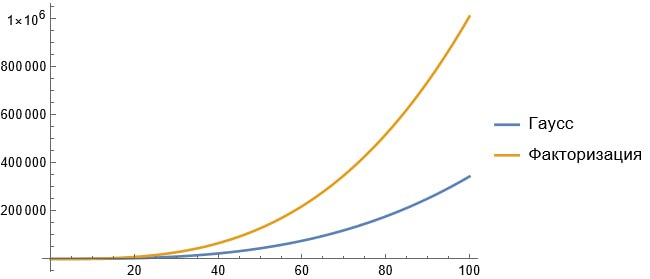
\includegraphics{GaussFactor}
		\caption{Сравнение количества операций}
	\end{figure}
	
	
	Видно, что факторизация требует больше операций чем метод Гаусса. Однако факторизация ищет более точное решение для плохо обусловленных матриц т.к. в прямом ходе метода Гаусса нужно делить на ведущий элемент в отличии от метода факторизации.
    \item Как можно объединить в одну процедуру прямой и обратный ход метода Гаусса? В чем достоинства и недостатки
    такого подхода?
    \newline
    {\bfseries Ответ}.
    Для объединения прямого и обратного хода Гаусса рассмотрим матрицу 
    система на $k$-ой итерации. Требуется выполнить одну итерацию прямого хода. Таким образом занулить элементы под главной диагональю, после занулить элементы над главной диагональю. Реализовать это можно следующим образом после прямого хода Гаусса можно транспонировать матрицу и запустить еще раз прямой ход Гаусса в итоге получим полностью диагональную матрицу. Данный метод будет требовать $\frac{n(n+1)(2n+1)}{3} = \frac{2}{3}n^3+n^2+\frac{n}{3}$ операций, а обычный метод Гаусса $\frac{n(n+1)(2n+1)}{6}+\frac{n(n-1)}{2}=\frac{n^3-n}{3}+n^2$. Таким образом данная процедура занимает больше операций чем обычный метод Гаусса. Смотреть схему ниже
	
	
	\[
	A = \begin{pmatrix}
		a_{11} & a_{12} & \ldots & a_{1k} & \ldots \\
		0 & a_{22} & \ldots & a_{2k} & \ldots \\
		0 & 0 & \ldots & \ldots & \ldots \\
		\ldots & \ldots & \ldots & a_{k-1,k} & \ldots \\
		0 & 0 &  \ldots & a_{k,k} & \ldots \\
		0 & 0 & \ldots & a_{k+1, k} & \ldots \\
		\ldots & \ldots & \ldots & \ldots & \ldots \\
		0 & 0 & \ldots & a_{n,k} & \ldots
	\end{pmatrix}
	\rightarrow
	\begin{pmatrix}
		a_{11} & a_{12} & \ldots & a_{1k} & \ldots \\
		0 & a_{22} & \ldots & a_{2k} & \ldots \\
		0 & 0 & \ldots & \ldots & \ldots \\
		\ldots & \ldots & \ldots & a_{k-1,k} & \ldots \\
		0 & 0 &  \ldots & a_{k,k} & \ldots \\
		0 & 0 & \ldots & 0 & \ldots \\
		\ldots & \ldots & \ldots & \ldots & \ldots \\
		0 & 0 & \ldots & 0 & \ldots
	\end{pmatrix}
	\rightarrow
	\begin{pmatrix}
		a_{11} & a_{12} & \ldots & 0 & \ldots \\
		0 & a_{22} & \ldots & 0 & \ldots \\
		0 & 0 & \ldots & \ldots & \ldots \\
		\ldots & \ldots & \ldots & 0 & \ldots \\
		0 & 0 &  \ldots & a_{k,k} & \ldots \\
		0 & 0 & \ldots & 0 & \ldots \\
		\ldots & \ldots & \ldots & \ldots & \ldots \\
		0 & 0 & \ldots & 0 & \ldots
	\end{pmatrix}
	\]
    \item Объясните, почему, говоря о векторах, норму $\|\cdot\|_1$ часто
    называют октаэдрической, норму $\|\cdot\|_2$ — шаровой, а норму
    $\|\cdot\|_\infty$ — кубической.
    \newline
    {\bfseries Ответ}.
    Для простоты в начале рассмотрим, при размерности пространства 2.
	
	
	
	\noindent 1)$||\cdot||_2$ — шаровая норма.
	
	
	Рассмотрим множество $S=\{\vec{x}: \, ||\vec{x}||_2 \le 1\}$. Раскроем норму по определению и получим $S=\{\vec{x}:\, x^2+y^2 \le 1\}$. Видно, что полученное множество является кругом.
	
	
	
	\begin{figure}[!h]
		\center
		\label{circle}
		\begin{tikzpicture}[scale=2]
			% Заштрихованный круг радиуса 1
			\filldraw[gray!30] (0,0) circle [radius=1];
			
			% Окружность
			\draw (0,0) circle [radius=1];
			
			% Оси координат
			\draw[->] (-1.5,0) -- (1.8,0) node[right] {$x$};
			\draw[->] (0,-1.5) -- (0,1.8) node[above] {$y$};
			
			% Точка на окружности
			\filldraw[black] (0.6, 0.8) circle (1.5pt) node[above right] {$(x, y)$};
			
			% Перпендикуляры к осям x и y
			\draw[dashed] (0.6, 0.8) -- (0.6, 0) node[below left] {$x$};
			\draw[dashed] (0.6, 0.8) -- (0, 0.8) node at (0.75, 0.4) {$y$}; % Переместил на катет
			
			% Прямая из начала координат к точке (0.6, 0.8)
			\draw[->, thick] (0,0) -- (0.6, 0.8) node[midway, sloped, above, font=\scriptsize] {$\sqrt{x^2 + y^2}$}; % Сделал еще меньше
			
			% Отметка радиуса
			\draw[red,->] (0,0) -- (1,0) node[below right] {$1$}; 
			
		\end{tikzpicture}
		\caption{$S=\{\vec{x}:\, x^2+y^2 \le 1\}$}
	\end{figure}
	
	
	
	\noindent 2)$||\cdot||_\infty$ — кубическая норма.
	Рассмотрим множество $S=\{\vec{x}: \, ||\vec{x}||_\infty \le 1\}$. 
    Раскроем норму по определению и получим $S=\{\vec{x}:\, max(|x|,|y|) \le 1\}$. 
    Видно, что полученное множество является квадратом со стороной 2.
	

	\begin{figure}[H]
		\center
		\label{square}
		\begin{tikzpicture}[scale = 1.5]
			% Заштрихованный квадрат со стороной 2
			\filldraw[gray!30] (-1,-1) rectangle (1,1);
			
			% Оси координат
			\draw[->] (-2,0) -- (2,0) node[right] {$x$};
			\draw[->] (0,-2) -- (0,2) node[above] {$y$};
			
			% Квадрат (чтобы был контур)
			\draw (-1,-1) rectangle (1,1);
			
			% Точка на квадрате (например, на верхней границе квадрата)
			\filldraw[] (0.5, 1) circle (1.5pt) node[above right] {$(x, y)$};
			
			% Перпендикуляры к осям x и y
			\draw[dashed] (0.5, 1) -- (0.5, 0) node[below] {$x$};
			\draw[dashed] (0.5, 1) -- (0, 1) node[left] {$y$};
			
			% Вектор из начала координат в точку на квадрате
			\draw[->, thick] (0,0) -- (0.5, 1);
			\draw[red,->] (0,0) -- (1,0) node[below right] {$1$}; 
		\end{tikzpicture}
		\caption{$S=\{\vec{x}:\, max(|x|,|y|) \le 1\}$}
	\end{figure}
	
	
	\noindent 3)$||\cdot||_1$ — октаэдрическая норма.
	Рассмотрим множество $S=\{\vec{x}: \, ||\vec{x}||_1 \le 1\}$. Раскроем норму по определению и получим $S=\{\vec{x}:\, |x|+|y| \le 1\}$. Например, когда $x>0, y>0$, то имеем $y \le 1-x$, данная область является область. под прямой $y=1-x$. Аналогично получаем, что данная область это правильный ромб со стороной 1.
	
	\begin{figure}[H]
		\center
		\label{romb}
		\begin{tikzpicture}
			% Заштрихованный ромб
			\filldraw[gray!30] (0,2) -- (2,0) -- (0,-2) -- (-2,0) -- cycle;
			
			% Оси координат
			\draw[->] (-3,0) -- (3,0) node[right] {$x$};
			\draw[->] (0,-3) -- (0,3) node[above] {$y$};
			
			% Контур ромба
			\draw (0,2) -- (2,0) -- (0,-2) -- (-2,0) -- cycle;
			
			% Точка на ромбе (например, на верхней границе ромба)
			\filldraw[] (0.5, 1.5) circle (1.5pt) node[above right] {$(x, y)$};
			
			% Перпендикуляры к осям x и y
			\draw[dashed] (0.5, 1.5) -- (0.5, 0) node[below] {$x$};
			\draw[dashed] (0.5, 1.5) -- (0, 1.5) node[left] {$y$};
			
			% Вектор из начала координат в точку на ромбе
			\draw[->, thick] (0,0) -- (0.5, 1.5);
			\draw[red,->] (0,0) -- (2,0) node[below right] {$1$}; 
		\end{tikzpicture}
		\caption{$S=\{\vec{x}:\, |x|+|y| \le 1\}$}
	\end{figure}
	
	
	
	Аналогичные области будут получаться в пространстве.
	
	\noindent 1)$||\cdot||_2$ — шаровая норма. Рассмотрим $S=\{\vec{x}:\, x^2+y^2+z^2 \le 1\}$. Данная область представляет собой сферу радиуса 1.
	
	\begin{figure}[H]
		\center
		\label{sfera}
		\begin{tikzpicture}[tdplot_main_coords, scale = 2.5]
			
			% Create a point (P)
			\coordinate (P) at ({1/sqrt(3)},{1/sqrt(3)},{1/sqrt(3)});
			
			% Draw shaded circle
			\shade[ball color = lightgray,
			opacity = 0.5
			] (0,0,0) circle (1cm);
			
			% draw arcs 
			\tdplotsetrotatedcoords{0}{0}{0};
			\draw[dashed,
			tdplot_rotated_coords,
			gray
			] (0,0,0) circle (1);
			
			
			% Projection of the point on X and y axes
			\draw[thin, dashed] (P) --++ (0,0,{-1/sqrt(3)});
			\draw[thin, dashed] ({1/sqrt(3)},{1/sqrt(3)},0) --++
			(0,{-1/sqrt(3)},0);
			\draw[thin, dashed] ({1/sqrt(3)},{1/sqrt(3)},0) --++
			({-1/sqrt(3)},0,0);
			
			% Axes in 3 d coordinate system
			\draw[-stealth] (0,0,0) -- (1.80,0,0);
			\draw[-stealth] (0,0,0) -- (0,1.30,0);
			\draw[-stealth] (0,0,0) -- (0,0,1.30);
			\draw[dashed, gray] (0,0,0) -- (-1,0,0);
			\draw[dashed, gray] (0,0,0) -- (0,-1,0);
			
			% Line from the origin to (P)
			\draw[thick, -stealth] (0,0,0) -- (P);
			
			% Add small circle at (P)
			\draw[fill = lightgray!50] (P) circle (0.5pt);
			
		\end{tikzpicture}
		\caption{$S=\{\vec{x}:\, x^2+y^2+z^2 \le 1\}$}
	\end{figure}
	
	
	\noindent 2)$||\cdot||_\infty$ — кубическая норма. Рассмотрим $S=\{\vec{x}:\, max(|x|,|y|,|z|) \le 1\}$. Данная область представляет собой куб со стороной 2.
	\begin{figure}[H]
		\center
		\begin{tikzpicture}[tdplot_main_coords]
			
			% Куб
			\draw[thick] (1,1,1) -- (1,-1,1) -- (-1,-1,1) -- (-1,1,1) -- cycle; % Верхний квадрат
			\draw[thick] (1,1,-1) -- (1,-1,-1) -- (-1,-1,-1) -- (-1,1,-1) -- cycle; % Нижний квадрат
			
			\draw[thick] (1,1,1) -- (1,1,-1);
			\draw[thick] (1,-1,1) -- (1,-1,-1);
			\draw[thick] (-1,-1,1) -- (-1,-1,-1);
			\draw[thick] (-1,1,1) -- (-1,1,-1);
			

			
		\end{tikzpicture}
		\caption{$S=\{\vec{x}:\, |x|+|y|+|z| \le 1\}$}
	\end{figure}
	
	\noindent 3)$||\cdot||_1$ — октаэдрическая норма. Рассмотрим $S=\{\vec{x}:\, |x|+|y|+|z| \le 1\}$. Данная область представляет собой правильный октаэдр со стороной 1.
	\begin{figure}[H]
		\center
		\begin{tikzpicture}
			\tikzstyle{point}=[circle,thick,draw=black,fill=black,inner sep=0pt,minimum width=1pt,minimum height=1pt]
			\node (a)[point] at (0,0) {};
			\node (b)[point] at (2,0) {};
			\node (c)[point] at (3,1) {};
			\node (d)[point] at (1,1) {};
			\node (e)[point] at (1.5,3) {};
			\node (f)[point] at (1.5,-2) {};
			\draw (a.center) -- (b.center) -- (c.center) -- (e.center) -- (b.center);
			\draw (a.center) -- (e.center);
			\draw[dashed] (a.center) -- (d.center) -- (c.center);
			\draw[dashed] (d.center) -- (e.center);
			
			\draw (a.center) -- (f.center) -- (b.center);
			\draw (f.center) -- (c.center);
			\draw[dashed] (f.center) -- (d.center);

		\end{tikzpicture}
		\caption{$S=\{\vec{x}:\, |x|+|y|+|z| \le 1\}$}
	\end{figure}
\end{enumerate}
\end{document}
